% Created 2023-04-13 Thu 16:59
% Intended LaTeX compiler: pdflatex
\documentclass[presentation,mathserif,table]{beamer}
\usepackage[utf8]{inputenc}
\usepackage[T1]{fontenc}
\usepackage{graphicx}
\usepackage{longtable}
\usepackage{wrapfig}
\usepackage{rotating}
\usepackage[normalem]{ulem}
\usepackage{amsmath}
\usepackage{amssymb}
\usepackage{capt-of}
\usepackage{hyperref}
\usepackage{minted}
\beamertemplatenavigationsymbolsempty
\usepackage[T1]{fontenc}
\usepackage{DejaVuSans}
\usepackage{DejaVuSansMono}
\usefonttheme{professionalfonts}
\usepackage[euler-digits,euler-hat-accent]{eulervm}
\setbeamertemplate{itemize items}{•}
\setbeamertemplate{enumerate items}[default]
\AtBeginSection[]
{
\begin{frame}<beamer>
\frametitle{Outline}
\tableofcontents[currentsection]
\end{frame}
}
\setcounter{tocdepth}{1}
\setbeamertemplate{headline}{}
\setbeamertemplate{footline}{
\leavevmode%
\hbox{%
\begin{beamercolorbox}[wd=\paperwidth,ht=2.25ex,dp=1ex,right]{fg=black}%
\usebeamerfont{section in head/foot}\insertsection\hspace*{2em}
\insertframenumber{} / \inserttotalframenumber\hspace*{2ex}
\end{beamercolorbox}%
}%
\vskip0pt%
}
\usepackage{appendixnumberbeamer}
\setbeamersize{text margin left=3mm,text margin right=3mm}
\newcommand\blfootnote[1]{%
\begingroup
\renewcommand\thefootnote{}\footnote{#1}%
\addtocounter{footnote}{-1}%
\endgroup
}
\setbeamerfont{footnote}{size=\tiny}
\usepackage{tikz}
\usepackage[retainorgcmds]{IEEEtrantools}
\hypersetup{colorlinks=true, allcolors=., urlcolor=blue}
\usepackage[absolute,overlay]{textpos}
\usepackage{xcolor}
\definecolor{LightGray}{gray}{0.96}
\usepackage{minted}
\setminted{bgcolor=LightGray, fontsize=\small}
\newcommand{\eg}{e.g.\,}
\newcommand{\ie}{i.e.\,}
\newcommand{\aka}{a.k.a.\,}
\newcommand{\etc}{\emph{etc.}\,}
\newcommand{\X}{{\mathbold X}}
\newcommand{\bS}{{\mathbold S}}
\newcommand{\bSigma}{{\mathbold \Sigma}}
\newcommand{\x}{{\mathbold x}}
\newcommand{\bbeta}{{\mathbold \beta}}
\newcommand{\Y}{{\mathbold Y}}
\newcommand{\y}{{\mathbold y}}
\newcommand{\B}{{\mathbold B}}
\newcommand{\W}{{\mathbold W}}
\newcommand{\U}{{\mathbold U}}
\newcommand{\V}{{\mathbold V}}
\newcommand{\bH}{{\mathbold H}}
\newcommand{\R}{\mathbb{R}}
\DeclareMathOperator*{\argmin}{argmin}
\DeclareMathOperator*{\argmax}{argmax}
\DeclareMathOperator*{\tv}{TV}
\DeclareMathOperator*{\Tr}{Tr}
\DeclareMathOperator*{\FFT}{FFT}
\DeclareMathOperator*{\IFFT}{IFFT}
\DeclareMathOperator*{\diag}{diag}
\DeclareMathOperator*{\supp}{supp}
\DeclareMathOperator*{\tf}{tf}
\DeclareMathOperator*{\idf}{idf}
\DeclareMathOperator*{\df}{df}
\DeclareMathOperator*{\Var}{Var}
\DeclareMathOperator*{\Frob}{Frob}
\DeclareMathOperator*{\F}{F}
\DeclareMathOperator*{\softmax}{softmax}
\DeclareMathOperator*{\AUC}{AUC}
\usepackage{bm}
\usecolortheme{dove}
\setbeamercolor*{block title example}{fg=black,bg=white}
\setbeamercolor*{block body example}{fg=black,bg=white}
\usetheme{default}
\author{Jerome Dockes}
\date{}
\title{Model selection and validation}
\author{Jérôme Dockès \& Nikhil Bhagwat}
\titlegraphic{
\includegraphics[height=1.5cm]{figures/mcgill-university.png} \hspace{1.5cm} 
\includegraphics[height=1.5cm]{figures/origami-lab-logo.png}}
\date{QLS 612 2023-05-04}
\hypersetup{
 pdfauthor={Jerome Dockes},
 pdftitle={Model selection and validation},
 pdfkeywords={},
 pdfsubject={},
 pdfcreator={Emacs 27.1 (Org mode 9.6.2)}, 
 pdflang={English}}
\begin{document}

\maketitle
\section{Introduction: cross-validation}
\label{sec:orgfaee4a9}
\subsection{Recap of part 1}
\label{sec:orga8d0ea3}
\begin{frame}[label={sec:orgb83bc1d}]{Recap of part 1}
\begin{block}{Supervised learning}
\begin{itemize}
\item Regression: least-squares linear regression
\item Classification: logistic regression
\end{itemize}
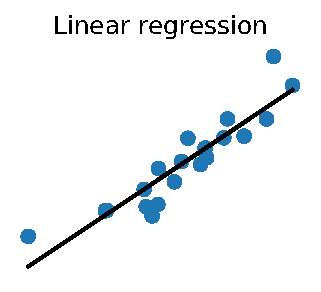
\includegraphics[height=.4 \textheight]{figures/generated/linear_regression_1d/linear_regression.pdf}
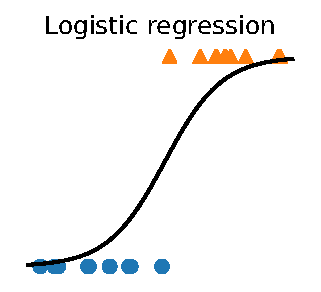
\includegraphics[height=.4 \textheight]{figures/generated/logistic_regression_1d/logistic_regression.pdf}
\end{block}
\end{frame}

\begin{frame}[label={sec:org9f9b470}]{Recap of part 1}
\begin{block}<1->{Supervised learning}
\begin{itemize}
\item Regression: least-squares linear regression
\item Classification: logistic regression
\end{itemize}
\end{block}
\begin{block}<1->{Regularization}
\begin{itemize}
\item \(\ell_2\) \aka ridge regularization
\end{itemize}
\end{block}
\begin{block}<2->{Model evaluation and selection}
\begin{itemize}
\item Out-of-sample generalization; independent test set
\item Performance metrics:
\begin{itemize}
\item regression: mean squared error
\item classification: accuracy, ROC curve
\end{itemize}
\item Cross-validation
\end{itemize}
\end{block}
\end{frame}
\begin{frame}[label={sec:orge4c2f8f}]{Notation \& vocabulary}
\begin{block}{Supervised learning framework}
\begin{equation}
Y = f(X) + E
\end{equation}
\vspace{-10pt}
\begin{itemize}[<+->]
\item \(Y \in \R\): output (\aka target, dependent variable) to predict
\item \(X \in \R^p\): features (\aka inputs, regressors, descriptors, independent variables)
\item \(E \in \R\): unmodelled noise
\item \(f\): the function we try to approximate
\end{itemize}
\end{block}
\begin{example}<4->[Linear regression]
\vspace{-20pt}
 \begin{IEEEeqnarray}{rCl}
 Y & = & \beta_0 + \langle X, \beta \rangle + E \\
& = & \beta_0 + \sum_{j=1}^p X_j \, \beta_j + E
 \end{IEEEeqnarray}
"learning" = choosing \(\beta_0 \in \R\) and \(\bbeta \in \R^p\)
\end{example}
\end{frame}
\begin{frame}[label={sec:org4ce6c43}]{How to set parameters: Empirical Risk Minimization}
\begin{itemize}
\item Choose a loss function \(L\) measuring how bad is our error.
\item Example: squared error \(L(Y, \hat{Y}) = (Y - \hat{Y})^2\), where \(\hat{Y}\) is the prediction
\item We want to minimize the expected error (risk): \(\mathbb{E}[L(Y, \hat{Y})]\)
\end{itemize}
\end{frame}
\begin{frame}[label={sec:orgb437980}]{How to set parameters: Empirical Risk Minimization}
We do not know the risk: estimate it from a sample.

Given \(n\) training examples \(\X \in \R^{n \times p}\), \(\y \in \R^n\),
minimize the empirical risk: \(\sum_{i=1}^n L(\y_i, \hat{\y_i})\)

\begin{block}{For linear regression:}
find \(\hat{\beta}_0 \in \R, \hat{\bbeta} \in \R^p\) that minimize
\begin{IEEEeqnarray}{rcl}
\| \y - \hat{\y} \|_2^2 & \; = \; & \| \y - \hat{\beta}_0 - \X \, \hat{\bbeta} \|_2^2 \\
& \; = \; & \sum_{i=1}^n (\y_i - \hat{\beta}_0 - \sum_{j=1}^p \X_{ij}\, \hat{\bbeta}_j )^2
\end{IEEEeqnarray}

"Fitting" the parameters to \(\X, \y\).
\end{block}
\end{frame}

\begin{frame}[label={sec:orgb64269e}]{Evaluating a model}
\begin{block}{We always want to do 2 distinct things:}
\begin{itemize}
\item Select a model (set the parameters).
\item Evaluate its performance.
\end{itemize}

\vfill
\end{block}

\begin{structureenv} %% warning
We can never do both on the same data!
\end{structureenv}
\end{frame}
\begin{frame}[label={sec:org3b41f14}]{Training error is a biased estimator of the risk}
\begin{itemize}
\item 30 different animals made predictions about match results in the 2022 World Cup
\end{itemize}
\begin{center}
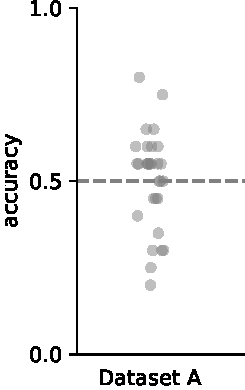
\includegraphics[height=.65 \textheight]{figures/generated/select_evaluate/select_evaluate_1.pdf}
\end{center}
\end{frame}
\begin{frame}[label={sec:org41917dd}]{Training error is a biased estimator of the risk}
\begin{itemize}
\item 30 different animals made predictions about match results in the 2022 world cup
\item We \alert{selected the best predictor} (highest accuracy)
\end{itemize}
\begin{center}
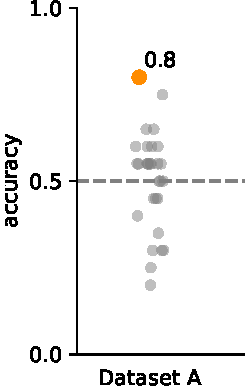
\includegraphics[height=.65 \textheight]{figures/generated/select_evaluate/select_evaluate_2.pdf}
\end{center}
\end{frame}
\begin{frame}[label={sec:org8301e08}]{Training error is a biased estimator of the risk}
The same animal is invited to make predictions about the 2026 World Cup.
Is it more likely to perform:
\begin{enumerate}
\item Better than in 2022?
\item Worse than in 2022?
\item The same?
\end{enumerate}
\begin{center}
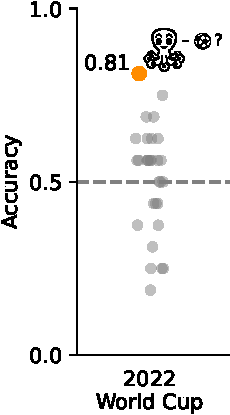
\includegraphics[height=.65 \textheight]{figures/generated/select_evaluate/select_evaluate_2b.pdf}
\end{center}
\end{frame}

\begin{frame}[label={sec:orgc24bf8c}]{Training error is a biased estimator of the risk}
The selected animal is more likely to perform \alert{worse} than in 2022.
\begin{center}
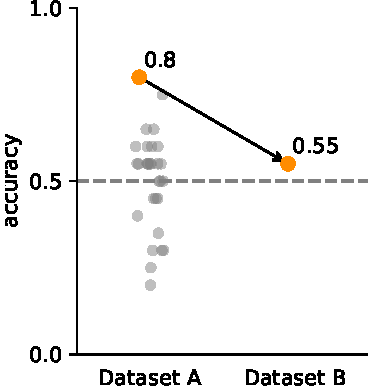
\includegraphics[height=.65 \textheight]{figures/generated/select_evaluate/select_evaluate_3.pdf}
\end{center}
\end{frame}
\begin{frame}[label={sec:org81f35bb}]{Training error is a biased estimator of the risk}
The selected animal is more likely to perform \alert{worse} than in 2022.
\begin{center}
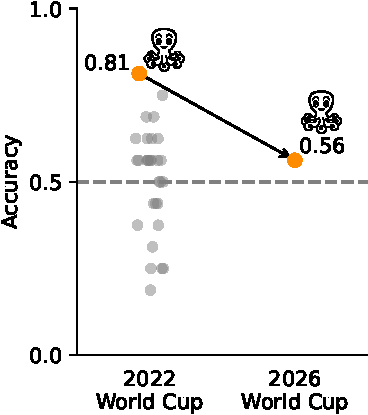
\includegraphics[height=.65 \textheight]{figures/generated/select_evaluate/select_evaluate_3b.pdf}
\end{center}
Its 2022 performance is a \alert{biased} estimator of its expected performance in future World Cups.
\end{frame}
\begin{frame}[label={sec:orgccf5df6}]{Training error is a biased estimator of the risk}
Distribution of train and test errors across 50 repetitions:
\begin{center}
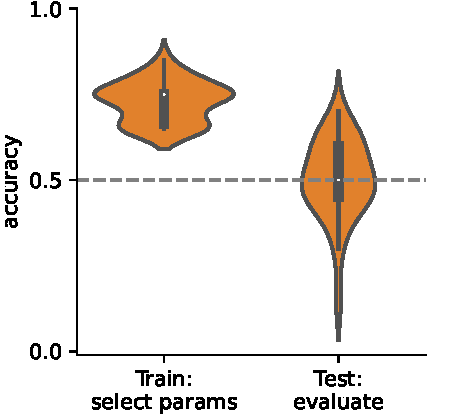
\includegraphics[height=.5 \textheight]{figures/generated/select_evaluate_averaged/select_evaluate_averaged_1.pdf}
\end{center}
\end{frame}
\begin{frame}[label={sec:orgb0a873b}]{Training error is a biased estimator of the risk}
\begin{itemize}
\item The systematic difference is the bias.
\item It is why we cannot use the training error to estimate model performance.
\end{itemize}
\begin{center}
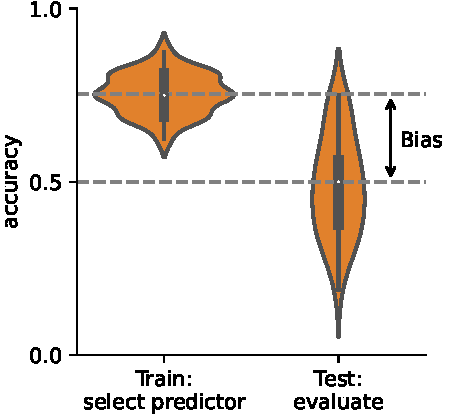
\includegraphics[height=.5 \textheight]{figures/generated/select_evaluate_averaged/select_evaluate_averaged_2.pdf}
\end{center}
\end{frame}


\begin{frame}[label={sec:org8120e4f}]{Estimating prediction performance}
When you hear "best", "maximum", "select", \ldots{} think "bias"
\begin{block}{Setting the parameters}
\begin{itemize}
\item \alert{Select} \(\bbeta\) that gives the \alert{best} prediction on training data
\item The prediction score for \(\hat{\bbeta}\) is biased: compute a new score on unseen test data.
\end{itemize}
\end{block}
\end{frame}
\subsection{Supervised learning with sklearn}
\label{sec:org1957bb4}
\begin{frame}[label={sec:org38fa8e3},fragile]{scikit-learn "estimator API": \texttt{fit; predict}}
 \begin{minted}[]{python}
estimator = Ridge()
estimator.fit(X_train, y_train)
predictions = estimator.predict(X_test)
\end{minted}
\vfill
\href{https://scikit-learn.org/stable/getting\_started.html}{Scikit-learn user guide}

\href{https://scikit-learn.org/stable/modules/generated/sklearn.linear\_model.Ridge.html}{\texttt{sklearn.linear\_model.Ridge}}

\vfill

("API": "Application Programming Interface" -- the specific way in which the library exposes its behaviour to user code: method names \& signatures, etc.)
\end{frame}
\begin{frame}[label={sec:org94826e7},fragile]{Evaluating performance with \texttt{sklearn.metrics}}
 \begin{minted}[]{python}
estimator = Ridge()
estimator.fit(X_train, y_train)
predictions = estimator.predict(X_test)

mse = metrics.mean_squared_error(y_test, predictions)
\end{minted}
\vfill

\href{https://scikit-learn.org/stable/modules/generated/sklearn.linear\_model.Ridge.html}{\texttt{sklearn.linear\_model.Ridge}}

\href{https://scikit-learn.org/stable/modules/classes.html\#module-sklearn.metrics}{\texttt{sklearn.metrics}}

\href{https://scikit-learn.org/stable/modules/model\_evaluation.html}{User guide on model evaluation}
\vfill
\href{https://github.com/neurodatascience/main-edu-courses-ml/tree/main/ml\_model\_selection\_and\_validation/exercises/ex\_01\_fit\_predict\_questions.py}{\texttt{ex\_01\_fit\_predict\_questions.py}}
\end{frame}

\begin{frame}[label={sec:org72cce59},fragile]{Some possible metrics for regression}
 \begin{block}{\(R^2\) score (coefficient of determination): \href{https://scikit-learn.org/stable/modules/model\_evaluation.html\#r2-score-the-coefficient-of-determination}{\texttt{r2\_score}}}
\begin{equation}
R^2(\y, \hat{\y}) = 1 - \frac{\sum_{i=1}^n(y_i  - \hat{y}_i)^2}{\sum_{i=1}^n(y_i  - \bar{y})^2} \; ,
\end{equation}
where \(\bar{y} = \frac{1}{n}\sum_{i=1}^n y_i\)
\end{block}

\begin{block}{Mean Squared Error (MSE): \href{https://scikit-learn.org/stable/modules/model\_evaluation.html\#mean-squared-error}{\texttt{mean\_squared\_error}}}
\begin{equation}
\text{MSE}(\y, \hat{\y}) = \frac{1}{n} \sum_{i=1}^n(y_i  - \hat{y}_i)^2
\end{equation}
\end{block}

\begin{block}{Mean Absolute Error (MAE): \href{https://scikit-learn.org/stable/modules/model\_evaluation.html\#mean-absolute-error}{\texttt{mean\_absolute\_error}}}
\begin{equation}
\text{MAE}(\y, \hat{\y}) = \frac{1}{n} \sum_{i=1}^n |y_i  - \hat{y}_i|
\end{equation}
\end{block}
\end{frame}

\subsection{cv}
\label{sec:org83b5f94}
\begin{frame}[label={sec:orgbb17ee9},fragile]{Cross-validation}
 \begin{center}
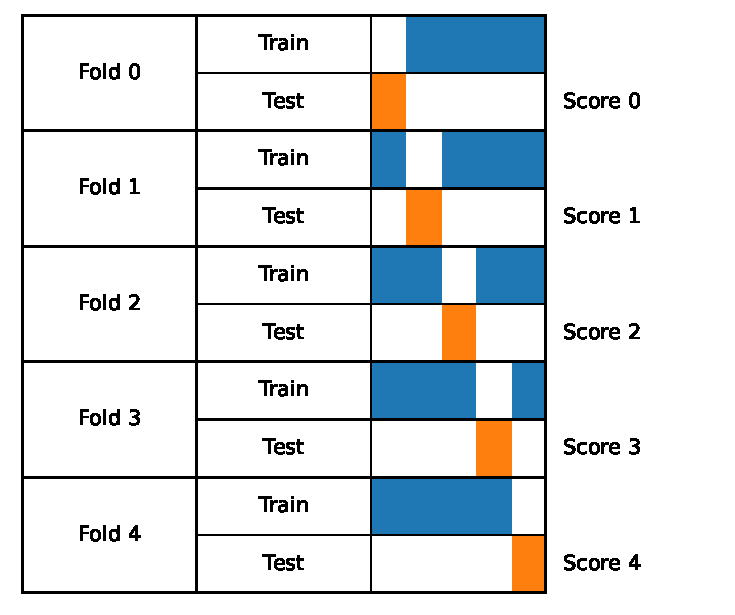
\includegraphics[height=.7 \textheight]{figures/generated/cv_figure_simple.pdf}
\end{center}

\vspace{-10pt}

\href{https://scikit-learn.org/stable/modules/cross\_validation.html}{User guide on cross-validation}
\href{https://scikit-learn.org/stable/modules/generated/sklearn.model\_selection.cross\_validate.html}{\texttt{sklearn.model\_selection.cross\_validate}}
\href{https://scikit-learn.org/stable/modules/generated/sklearn.model\_selection.cross\_val\_score.html}{\texttt{sklearn.model\_selection.cross\_val\_score}}
\href{https://github.com/neurodatascience/main-edu-courses-ml/tree/main/ml\_model\_selection\_and\_validation/exercises/ex\_02\_cross\_validate\_questions.py}{\texttt{ex\_02\_cross\_validate\_questions.py}}
\end{frame}
\section{Model and hyperparameter selection}
\label{sec:org9f48169}
\subsection{nested cv}
\label{sec:org5f8d63b}
\begin{frame}[label={sec:org5e7925e}]{Need for regularization}
Linear regression: projection on the column space of \(X\)
\vspace{10pt}
\begin{structureenv} %% top
\begin{columns}
\begin{column}{.3\columnwidth}
\begin{equation}
\hat{\y} = \X \, \hat{\bbeta}
\end{equation}
\end{column}

\begin{column}{.7\columnwidth}
\vspace{-17pt}
\begin{center}
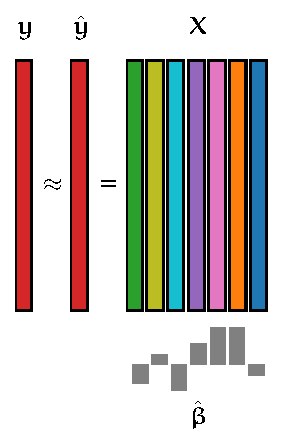
\includegraphics[height=.7\textheight]{figures/generated/dim_reduction_colors/regression_full_3.pdf}
\end{center}
\end{column}
\end{columns}
\end{structureenv}

\begin{structureenv} %% bottom
\begin{itemize}
\item Too many features: high variance \& unstable solution
\item Solutions: \alert{regularization}, dimensionality reduction
\end{itemize}
\end{structureenv}
\end{frame}
\begin{frame}[label={sec:orga58a1e8}]{Regularization}
\begin{example}[Ridge regression]
\begin{equation}
\argmin_{\bbeta, \beta_0} \| \y - \beta_0 - \X \, \bbeta \|_2^2 + \alpha \, \|\bbeta\|_2^2
\end{equation}
\end{example}
\end{frame}
\begin{frame}[label={sec:org25a03cf}]{}
\begin{columns}
\begin{column}{.33\columnwidth}
\(\small{ \text{Var}(\hat{\beta}_i) = \mathbb{E}(\hat{\beta}_i  - \mathbb{E}(\hat{\beta}_i))^2}\)
\end{column}

\begin{column}{.38\columnwidth}
\vspace{-15pt}
\begin{center}
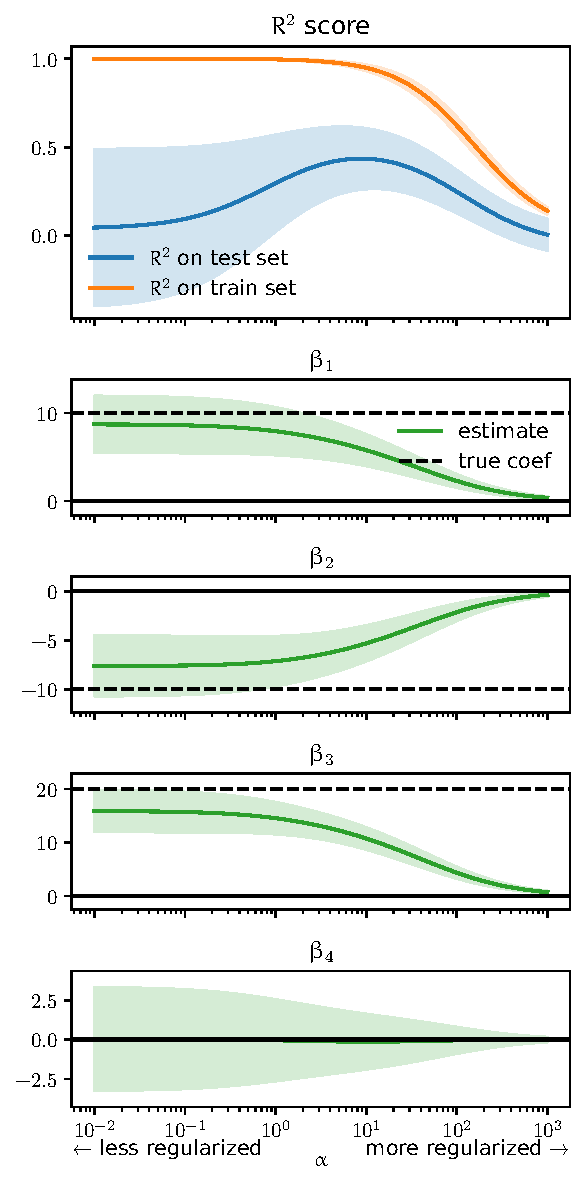
\includegraphics[height=\textheight]{figures/generated/ridge_regularization_path/ridge_regularization_path.pdf}
\end{center}
\end{column}
\begin{column}{.3\columnwidth}
\(\small \text{Bias}(\hat{\beta}_i) = \mathbb{E}(\hat{\beta}_i) - \beta_i\)
\end{column}
\end{columns}
\end{frame}

\begin{frame}[label={sec:orga0cc3a0}]{Setting hyperparameters}
\begin{block}{How can we choose the ridge hyperparameter \(\alpha\)?}
\end{block}
Try a few and pick the best one\ldots{}

But measure its performance on separate data!
\end{frame}
\begin{frame}[label={sec:org3733f3d}]{Nested cross-validation}
When you hear "best", "maximum", "select", \ldots{} think "bias"
\begin{block}<2->{Setting the parameters}
\begin{itemize}
\item \alert{Select} \(\bbeta\) that gives the \alert{best} prediction on training data
\item The prediction score for \(\hat{\bbeta}\) is biased: compute a new score on unseen test data.
\end{itemize}
\end{block}
\begin{block}<3->{Setting the hyperparameters}
\begin{itemize}
\item Repeat step 1 for a few values of \(\alpha\), fitting and testing several models
\item \alert{Select} the hyperparameter that obtains the \alert{best} prediction on test data
\item The prediction score of that model on \emph{test} data is biased: evaluate it again on unseen data
\end{itemize}
\end{block}
\end{frame}
\begin{frame}[label={sec:org7691605}]{One split}
\begin{center}
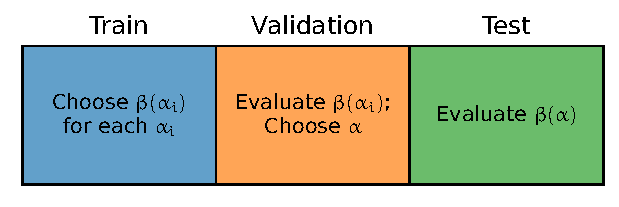
\includegraphics[width=.9\linewidth]{figures/generated/train_eval_test/datasets.pdf}
\end{center}
\end{frame}
\begin{frame}[label={sec:orgdf661b9},fragile]{Nested cross-validation}
 \begin{center}
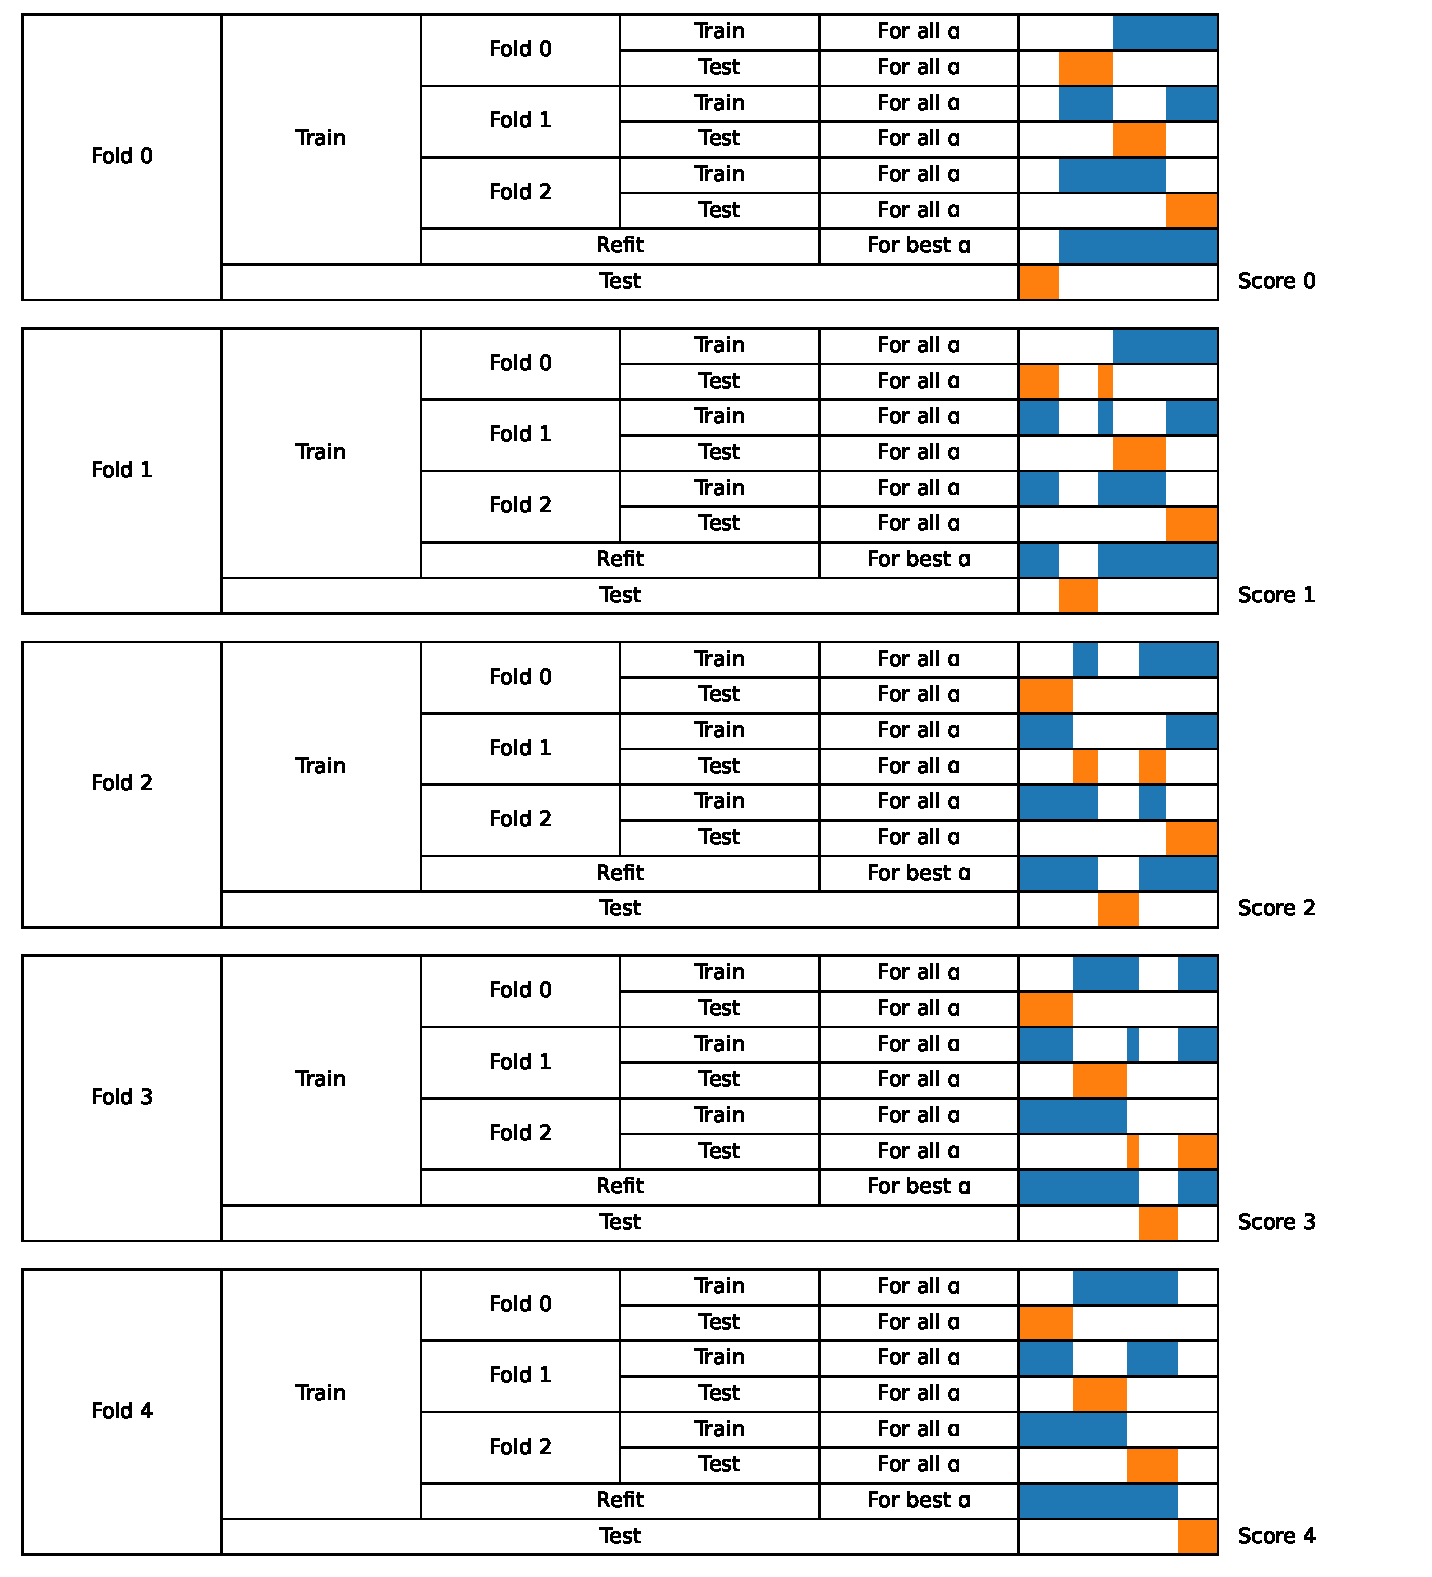
\includegraphics[width=.9\linewidth]{figures/generated/cv_figure_nested.pdf}
\end{center}
  see  \href{https://scikit-learn.org/stable/modules/generated/sklearn.model\_selection.GridSearchCV.html}{\texttt{sklearn.model\_selection.GridSearchCV}}
\end{frame}

\begin{frame}[label={sec:orgb9c6e63},fragile]{Nested cross-validation with scikit-learn}
 \begin{itemize}
\item In general: \href{https://scikit-learn.org/stable/modules/generated/sklearn.model\_selection.GridSearchCV.html}{\texttt{GridSearchCV}} (\href{https://scikit-learn.org/stable/modules/grid\_search.html\#grid-search}{User Guide})
\end{itemize}
\vfill
\begin{minted}[]{python}
model = GridSearchCV(
    Ridge(), {"alpha": [.1, 1., 10.]})
scores = cross_val_score(model, X, y)
\end{minted}
\vfill
\begin{itemize}
\item Use \href{https://scikit-learn.org/stable/glossary.html\#term-cross-validation-estimator}{CV estimators} when possible: \href{https://scikit-learn.org/stable/modules/generated/sklearn.linear\_model.RidgeCV.html}{\texttt{RidgeCV}}, \href{https://scikit-learn.org/stable/modules/generated/sklearn.linear\_model.LassoCV.html}{\texttt{LassoCV}}, \ldots{}
\end{itemize}

\vfill

\href{https://github.com/neurodatascience/main-edu-courses-ml/tree/main/ml\_model\_selection\_and\_validation/exercises/ex\_03\_grid\_search\_regression\_questions.py}{\texttt{ex\_03\_grid\_search\_regression\_questions.py}}
\end{frame}
\begin{frame}[label={sec:orge5bc777},fragile]{Implementing nested CV}
 \href{https://github.com/neurodatascience/main-edu-courses-ml/tree/main/ml\_model\_selection\_and\_validation/exercises/ex\_04\_nested\_cross\_validation\_questions.py}{\texttt{ex\_04\_nested\_cross\_validation\_questions.py}}
\end{frame}
\section{Dimensionality reduction}
\label{sec:org70e41ed}
\subsection{Intro}
\label{sec:org24711f5}
\begin{frame}[label={sec:org8511d63}]{Dimensionality reduction}
Linear regression: projection on the column space of \(X\)
\vspace{10pt}
\begin{structureenv} %% top
\begin{columns}
\begin{column}{.3\columnwidth}
\begin{equation}
\hat{\y} = \X \, \hat{\bbeta}
\end{equation}
\end{column}

\begin{column}{.7\columnwidth}
\vspace{-17pt}
\begin{center}
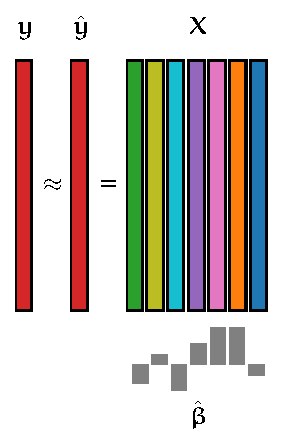
\includegraphics[height=.7\textheight]{figures/generated/dim_reduction_colors/regression_full_3.pdf}
\end{center}
\end{column}
\end{columns}
\end{structureenv}

\begin{structureenv} %% bottom
\begin{itemize}
\item Too many features: high variance \& unstable solution
\item Solutions: regularization, \alert{dimensionality reduction}
\end{itemize}
\end{structureenv}
\end{frame}
\begin{frame}[label={sec:orgd8244f4}]{Dimensionality reduction}
\begin{block}{Until now}
\begin{center}
\includegraphics[height=.12 \textheight]{figures/graphs/pipeline-1.pdf}
\end{center}
\end{block}
\begin{block}{Add a step in the pipeline: simplifying the inputs}
\begin{center}
\includegraphics[height=.12 \textheight]{figures/graphs/pipeline-2.pdf}
\end{center}
\end{block}
\end{frame}
\begin{frame}[label={sec:orgea60c31},fragile]{Simulated data for linear regression}
 \begin{itemize}
\item Generate \(\X \in \R^{n \times 3}\), \(\mathbold{\bbeta} \in \R^3\), \(\mathbold{e} \in \R^n\) and \(\y = \X \, \bbeta + \mathbold{e} \in R^n\)
\item Append columns containing random noise to \(\X\)
\item Now \(\X \in \R^{n \times p}\), with \(p \geq 3\), but only the first 3 columns are linked with \(\y\)
\item Split into training and testing tests and evaluate a linear regression model: what happens when \(p\) becomes large?
\end{itemize}

See \href{https://scikit-learn.org/stable/modules/generated/sklearn.datasets.make\_regression.html\#sklearn.datasets.make\_regression}{\texttt{sklearn.datasets.make\_regression}} for generating data
\begin{center}
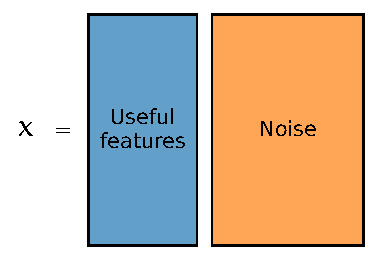
\includegraphics[height=.4 \textheight]{figures/generated/show_make_regression/x_construction.pdf}
\end{center}
\end{frame}
\begin{frame}[label={sec:org2aca4c8}]{Model complexity: overfitting}
\begin{itemize}
\item Model complexity increases with dimension.
\item Example: a linear model in dimension \(p\) can fit exactly (0 training error) any set of \(p + 1\) points.
\item Risk of overfitting: fitting exactly training data but failing on test data
\end{itemize}

\begin{center}
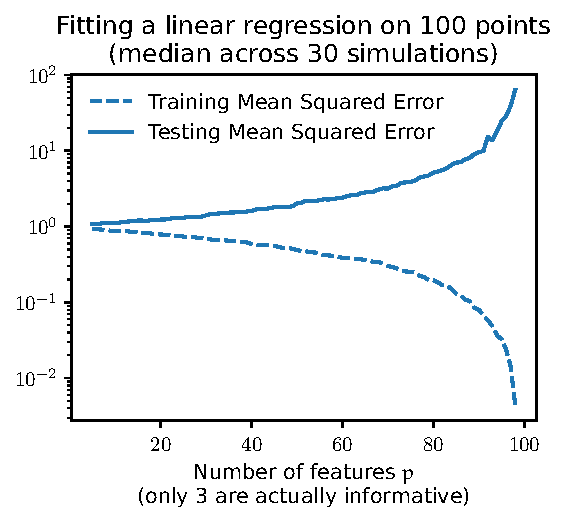
\includegraphics[height=.7\textheight]{figures/generated/ridge_overfitting/mse_log.pdf}
\end{center}
\end{frame}
\subsection{Univariate feature selection}
\label{sec:org5984507}
\begin{frame}[label={sec:org0b755bb}]{Univariate feature selection}
\begin{itemize}
\item \aka feature screening, filtering \ldots{}
\item Check features (columns of \(\X\)) one by one for association with the output \(\y\)
\item Keep only a fixed number or percentage of the features
\end{itemize}

\begin{block}{Simple (linear) association criteria}
\begin{itemize}
\item for regression: correlation
\item for classification: ANalysis Of VAriance
\end{itemize}
\end{block}
\begin{block}{Read more in the scikit-learn user guide}
\href{https://scikit-learn.org/stable/modules/feature\_selection.html\#feature-selection}{scikit-learn feature selection}
\end{block}
\end{frame}

\begin{frame}[label={sec:orgf26cb5a}]{Original regression problem}
\begin{columns}
\begin{column}{.3\columnwidth}
\begin{equation}
\hat{\y} = \X \, \hat{\bbeta}
\end{equation}
\end{column}

\begin{column}{.7\columnwidth}
\vspace{-17pt}
\begin{center}
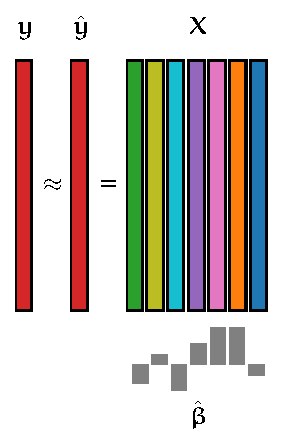
\includegraphics[height=.7\textheight]{figures/generated/dim_reduction_colors/regression_full_3.pdf}
\end{center}
\end{column}
\end{columns}
\end{frame}
\begin{frame}[label={sec:orga8fdb94}]{After univariate feature selection}
\begin{columns}
\begin{column}{.3\columnwidth}
\begin{equation}
\hat{\y} = \X \, \hat{\bbeta}
\end{equation}
\end{column}

\begin{column}{.7\columnwidth}
\vspace{-17pt}
\begin{center}
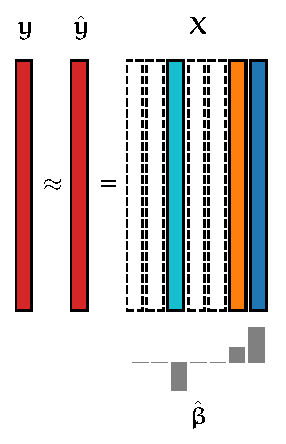
\includegraphics[height=.7\textheight]{figures/generated/feature_selection_colors/regression_selected_3_full_coef.pdf}
\end{center}
\end{column}
\end{columns}
\end{frame}

\begin{frame}[label={sec:orgcb38479}]{After univariate feature selection}
\begin{columns}
\begin{column}{.3\columnwidth}
\begin{equation}
\hat{\y} = \X \, \hat{\bbeta}
\end{equation}
\end{column}

\begin{column}{.7\columnwidth}
\vspace{-17pt}
\begin{center}
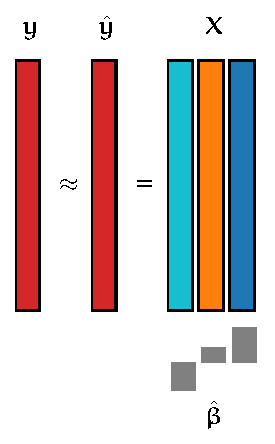
\includegraphics[height=.7\textheight]{figures/generated/feature_selection_colors/regression_selected_3.pdf}
\end{center}
\end{column}
\end{columns}
\end{frame}

\begin{frame}[label={sec:org3698c33}]{Univariate feature selection}
Keeping only the 10 best features (most correlated with \(\y\))
\begin{center}
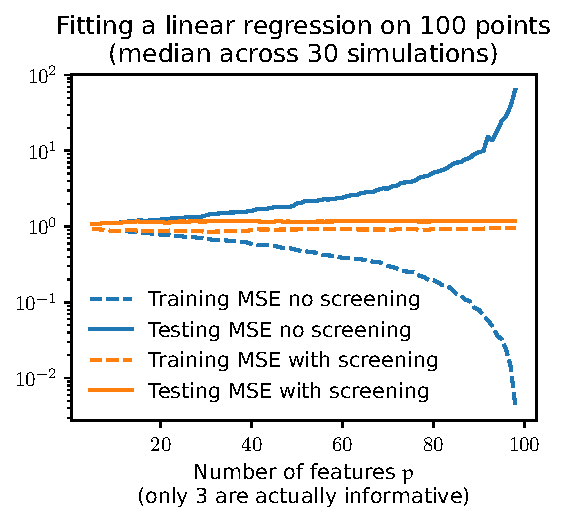
\includegraphics[height=.7\textheight]{figures/generated/ridge_overfitting/mse_with_dim_reduction_log.pdf}
\end{center}
\end{frame}

\subsection{Fit whole pipeline on train data only}
\label{sec:org98059ce}
\begin{frame}[label={sec:org3bc322a}]{Dataset transformations}
\begin{block}{Typical pipeline}
\begin{center}
\includegraphics[width=.9\linewidth]{figures/graphs/pipeline-2-no-color.pdf}
\end{center}
\end{block}
\begin{block}{Example}
\begin{center}
\includegraphics[width=.9\linewidth]{figures/graphs/pipeline-3.pdf}
\end{center}
\end{block}
\end{frame}
\begin{frame}[label={sec:org6c085e8},fragile]{scikit-learn "transformer API": \texttt{fit; transform}}
 \begin{minted}[]{python}
transformer = SelectKBest()
transformer.fit(X_train, y_train)
transformed_train = transformer.transform(X_train)
\end{minted}
\begin{block}{can also be written:}
\begin{minted}[]{python}
transformer = SelectKBest()
transformed_train = transformer.fit_transform(
    X_train, y_train)
\end{minted}
\end{block}
\begin{structureenv} %% links
\vfill

\href{https://scikit-learn.org/stable/modules/feature\_selection.html}{scikit-learn feature selection}

\href{https://scikit-learn.org/stable/getting\_started.html\#transformers-and-pre-processors}{scikit-learn \texttt{Transformer} API}
  \vfill
\end{structureenv}
\end{frame}

\begin{frame}[label={sec:orgda59d7c},fragile]{\texttt{feature\_selection.SelectKBest}}
 \begin{block}{\texttt{fit:}}
\begin{itemize}
\item compute ANOVA or correlation for each column of \(X\)
\item Remember the indices of the \(k\) columns with highest scores
\end{itemize}
\end{block}
\begin{block}{\texttt{transform:}}
\begin{itemize}
\item Index input to keep only the \(k\) selected columns
\end{itemize}
\end{block}


\begin{structureenv} %% link
\href{https://scikit-learn.org/stable/modules/generated/sklearn.feature\_selection.SelectKBest.html\#sklearn.feature\_selection.SelectKBest}{\texttt{sklearn.feature\_selection.SelectKBest}}
\end{structureenv}
\end{frame}



\begin{frame}[label={sec:orgf3668b3},fragile]{Fit the transformer only on train data!}
 \begin{minted}[]{python}
transformer = SelectKBest()
transformed_train = transformer.fit_transform(
    X_train, y_train)

transformed_test = transformer.transform(X_test)
\end{minted}
\end{frame}

\begin{frame}[label={sec:orgafa3251},fragile]{Pipelines}
 To chain transformations and an estimator, use \href{https://scikit-learn.org/stable/modules/generated/sklearn.pipeline.Pipeline.html}{\texttt{sklearn.pipeline.Pipeline}}

\begin{itemize}
\item can be used to properly cross-validate whole pipeline
\item can be combined with \texttt{cross\_validate}, \texttt{GridSearchCV}, \ldots{}
\item easily created with \href{https://scikit-learn.org/stable/modules/generated/sklearn.pipeline.make\_pipeline.html}{\texttt{sklearn.pipeline.make\_pipeline}}
\end{itemize}

\begin{minted}[]{python}
model = make_pipeline(SelectKBest(), Ridge())
\end{minted}
\begin{structureenv} %% links
\vfill
\href{https://github.com/neurodatascience/main-edu-courses-ml/tree/main/ml\_model\_selection\_and\_validation/exercises/ex\_05\_feature\_selection\_questions.py}{\texttt{ex\_05\_feature\_selection\_questions.py}}
\end{structureenv}
\end{frame}
\subsection{Linear decomposition methods}
\label{sec:orgcc14f53}
\begin{frame}[label={sec:org1e5a7cd}]{Linear decomposition methods}
Another approach to dimensionality reduction
\begin{block}{Maybe OK to drop \(\X_2\):}
\vspace{-10pt}
\begin{center}
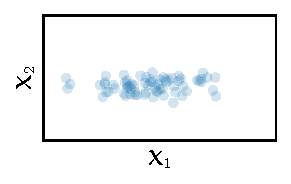
\includegraphics[height=.3\textheight]{figures/generated/pca/cloud_aligned.pdf}
\end{center}
\vspace{-20pt}
\end{block}
\begin{block}{Data low-dimensional but no feature can be dropped:}
\begin{center}
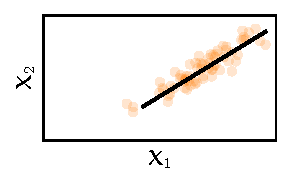
\includegraphics[height=.3\textheight]{figures/generated/pca/cloud_not_aligned.pdf}
\end{center}

Find a better referential in which to represent the data
\end{block}
\end{frame}
\begin{frame}[label={sec:orgd469c7f}]{Linear regression: projection on the column space of \(X\)}
\begin{structureenv} %% top
\begin{columns}
\begin{column}{.3\columnwidth}
\begin{equation}
\hat{\y} = \X \, \hat{\bbeta}
\end{equation}
\end{column}

\begin{column}{.7\columnwidth}
\vspace{-17pt}
\begin{center}
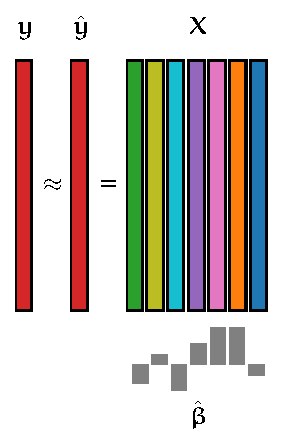
\includegraphics[height=.7\textheight]{figures/generated/dim_reduction_colors/regression_full_3.pdf}
\end{center}
\end{column}
\end{columns}
\end{structureenv}

\begin{structureenv} %% bottom
\begin{itemize}
\item Too many features: high variance \& unstable solution
\item Feature selection: drop some columns of \(\X\)
\item Other ways to build a family of \(k\) vectors on which to regress \(\y\)?
\end{itemize}
\end{structureenv}
\end{frame}
\begin{frame}[label={sec:org37f20ab}]{Linear decomposition: low-rank approximation of \(\X\)}
Minimize
\begin{equation}
\| \X - \W \, \bH \|_{\F}^2 = \sum_{i, j} ( \X_{i,j} - (\W \, \bH)_{i,j})^2
\end{equation}
\begin{center}
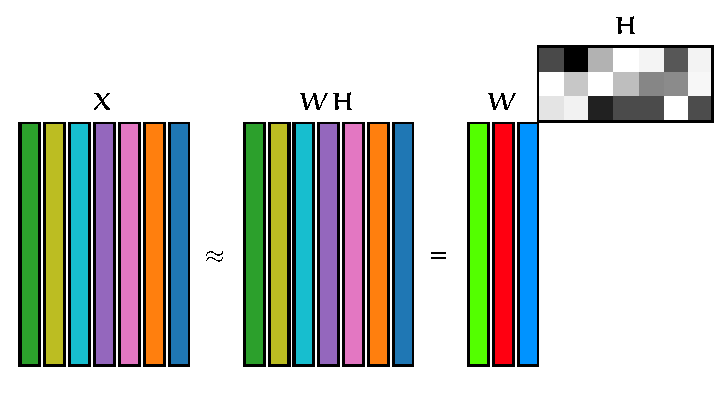
\includegraphics[height=.5\textheight]{figures/generated/dim_reduction_colors/factorization_3.pdf}
\end{center}
\end{frame}
\begin{frame}[label={sec:org8c1c091}]{Linear regression after dimensionality reduction}
\begin{equation}
\hat{\y} = \W \, \hat{\bbeta}
\end{equation}
\begin{center}
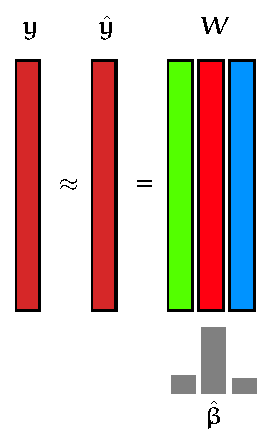
\includegraphics[height=.7\textheight]{figures/generated/dim_reduction_colors/regression_reduced_3.pdf}
\end{center}
\end{frame}
\begin{frame}[label={sec:orgd644ecc}]{Prediction for a new data point \(\x \in \R^{p}\)}
\begin{itemize}
\item Find the combination of rows of \(\bH\) that is closest to \(\x\): regress \(\x\) on \(\bH^T\)
\item Multiply by \(\hat{\bbeta}\)
\end{itemize}
    \begin{equation}
\x \in \R^p \rightarrow \text{projection} \rightarrow \mathbold{w} \in \R^k \rightarrow \langle \cdot \, , \, \hat{\bbeta}\rangle \rightarrow \hat{y} \in \R
    \end{equation}
\end{frame}
\begin{frame}[label={sec:orgf3d4b99}]{Principal Component Analysis}
\begin{itemize}
\item Singular Value Decomposition of \(\X\):
\end{itemize}
\begin{equation}
\X = \U \, \bS \, \V^T
\end{equation}
with \(\X \in \R^{n \times p}\), \(\U \in \R^{n \times r}\), \(\bS \in \R^{r \times r}\), \(\V \in \R^{r \times p}\)
\begin{itemize}
\item \(r = \min(n, p)\)
\item \(\bS \succeq 0\) diagonal with decreasing values \(s_j\) along the diagonal
\item \(\U^T\, \U = I_r\)
\item \(\V^T\, \V = I_r\)
\end{itemize}

Truncating the SVD to keep only the first \(k\) components gives the best rank-\(k\) approximation of \(\X\)
\begin{center}
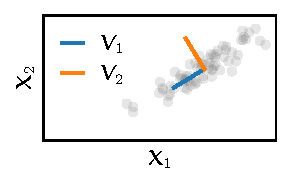
\includegraphics[height=.3\textheight]{figures/generated/pca/cloud_not_aligned_with_pc.pdf}
\end{center}
\end{frame}
\begin{frame}[label={sec:org0204479}]{Singular Value Decomposition}
\begin{equation}
\X = \U \, \bS \, \V^T
\end{equation}
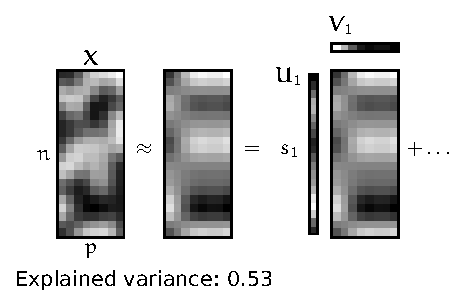
\includegraphics[height=.5 \textheight]{figures/generated/pca_step_by_step/pca_steps_1.pdf}

\begin{equation}
\U^T \, \U = I_p
\end{equation}
\begin{equation}
\V^T \, \V = I_p
\end{equation}
\end{frame}

\begin{frame}[label={sec:orgeb7a779}]{Singular Value Decomposition}
\begin{equation}
\X = \U \, \bS \, \V^T
\end{equation}
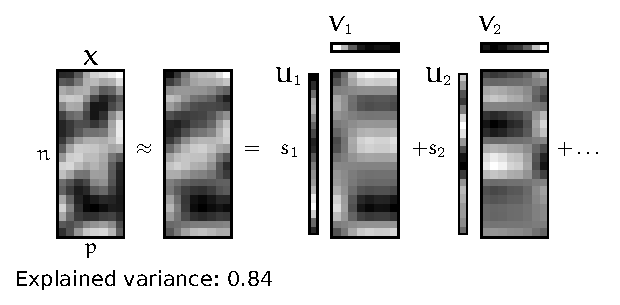
\includegraphics[height=.5 \textheight]{figures/generated/pca_step_by_step/pca_steps_2.pdf}

\begin{equation}
\U^T \, \U = I_p
\end{equation}
\begin{equation}
\V^T \, \V = I_p
\end{equation}
\end{frame}


\begin{frame}[label={sec:orgcc1a83b}]{Singular Value Decomposition}
\begin{equation}
\X = \U \, \bS \, \V^T
\end{equation}
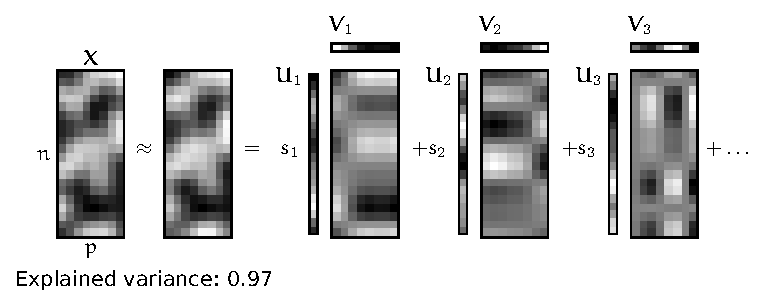
\includegraphics[height=.5 \textheight]{figures/generated/pca_step_by_step/pca_steps_3.pdf}

\begin{equation}
\U^T \, \U = I_p
\end{equation}
\begin{equation}
\V^T \, \V = I_p
\end{equation}
\end{frame}

\begin{frame}[label={sec:org2ab2ee6}]{Other decomposition methods}
Many other methods use the same objective (sum of squared reconstruction errors), but add penalties or constraints on the factors
\begin{itemize}
\item Dictionary Learning
\item Non-negative Matrix Factorization
\item K-means clustering
\item \ldots{}
\end{itemize}

\begin{block}{What about \(\y\)?}
\begin{itemize}
\item PCA is an example of \emph{unsupervised} learning: it does not use \(\y\)
\item Some other methods take it into account: \eg Partial Least Squares
\end{itemize}
\end{block}
\end{frame}
\begin{frame}[label={sec:org63a3e7b}]{Ridge regression and PCA}
\begin{itemize}
\item Both ridge regression and PC regression compute the coordinates of \(\y\) in the basis given by the SVD of \(\X\)
\item Ridge shrinks the coordinate along \(\U_j\) by a factor \(s_j^2 / (s_j^2 + \alpha)\)
\item PC regression sets the coordinates to 0 except for those corresponding to the \(k\) largest \(s_j\): shrinks by a factor \(\mathbold{1}_{\{j \leq k\}}\)
\end{itemize}

\begin{center}
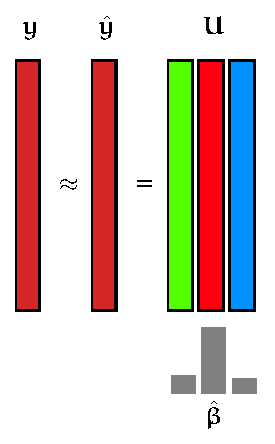
\includegraphics[height=.6\textheight]{figures/generated/dim_reduction_colors/regression_reduced_3_svd.pdf}
\end{center}
\end{frame}
\section{Conclusion: summary of pitfalls}
\label{sec:org38220b9}
\begin{frame}[label={sec:org6e70eed}]{(Cross-)validation experiments are simulations}
The validation experiments must simulate what will happen when deploying the trained model in production -- when starting to use it in real life.
\end{frame}
\begin{frame}[label={sec:org21ad79c}]{(Cross-)validation experiments are simulations}
The validation experiments must simulate what will happen when deploying the trained model in production -- when starting to use it in real life.
\begin{example}[Deploying a model to a hospital]
A model is trained on research dataset and then shipped and used on a hospital's patients.
We cannot:
\begin{itemize}
\item Preprocess the patients' data together with the training data.
\item Use the patients' data for feature selection.
\item Try different models on the patients' data and pick the best.
\end{itemize}

If we do any of these things in our cross-validation it is not a realistic experiment.
\end{example}
\end{frame}
\begin{frame}[label={sec:orgc0abca0}]{Split choice example: time series}
Don't ignore dependencies between samples: which is easier?
\begin{center}
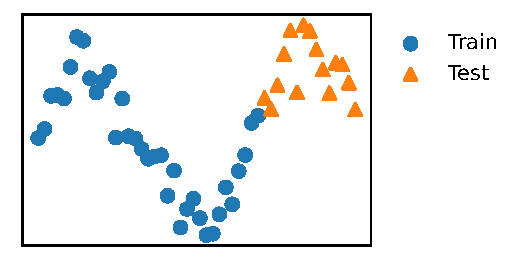
\includegraphics[height=.3 \textheight]{figures/generated/time_series_cv/kfold.pdf}
\end{center}

\begin{center}
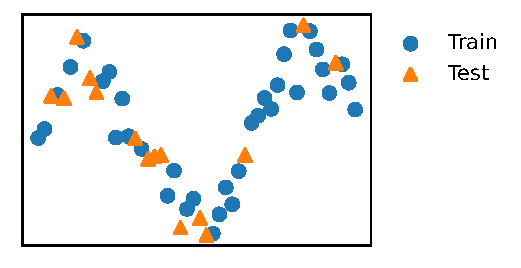
\includegraphics[height=.3 \textheight]{figures/generated/time_series_cv/kfold_shuffled.pdf}
\end{center}

Use the appropriate \href{https://scikit-learn.org/stable/modules/cross\_validation.html\#cross-validation-iterators}{cross-validation iterator}
\end{frame}
\begin{frame}[label={sec:org82f8be5}]{Remember that CV training sets overlap}
\begin{center}
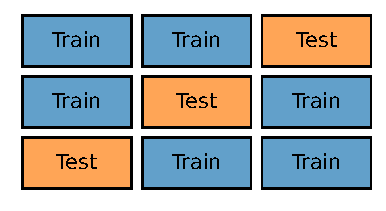
\includegraphics[height=.6 \textheight]{figures/generated/train_eval_test/cv_not_nested.pdf}
\end{center}

So the scores are not independent! Their variance can be underestimated.
\end{frame}

\begin{frame}[label={sec:org5dc78af},fragile]{Some pitfalls with cross-validation}
 \small
\begin{block}{Overfitting the hyperparameters}
\begin{itemize}
\item select hyperparameters with nested CV \href{https://scikit-learn.org/stable/modules/generated/sklearn.model\_selection.GridSearchCV.html}{\texttt{sklearn.model\_selection.GridSearchCV}}
\end{itemize}
\end{block}
\begin{block}{Fitting part of the pipeline on the whole dataset}
\begin{itemize}
\item use  \href{https://scikit-learn.org/stable/modules/generated/sklearn.pipeline.Pipeline.html}{\texttt{sklearn.pipeline.Pipeline}}
\end{itemize}
\end{block}
\begin{block}{Ignoring dependencies between samples}
\begin{itemize}
\item e.g. time series: use appropriate \href{https://scikit-learn.org/stable/modules/cross\_validation.html\#cross-validation-iterators}{cross-validation iterator}
\end{itemize}
\end{block}
\begin{block}{Ignoring dependencies between CV scores}
\begin{itemize}
\item Training sets overlap: cross-validation scores of different splits are not independent
\end{itemize}
\end{block}
\begin{block}{Over-interpreting good CV scores}
\end{block}
\end{frame}
\end{document}